\chapter{Evolution of the simulator}
	Equation \ref{eq:numerical_idm} can be solved with an Explicit Euler. To test the model a basic setup was implemented in MATLAB. The visual representation of the setup can be seen on figure \ref{fig:basic2car}.
	\begin{figure}[ht]
		\centering
		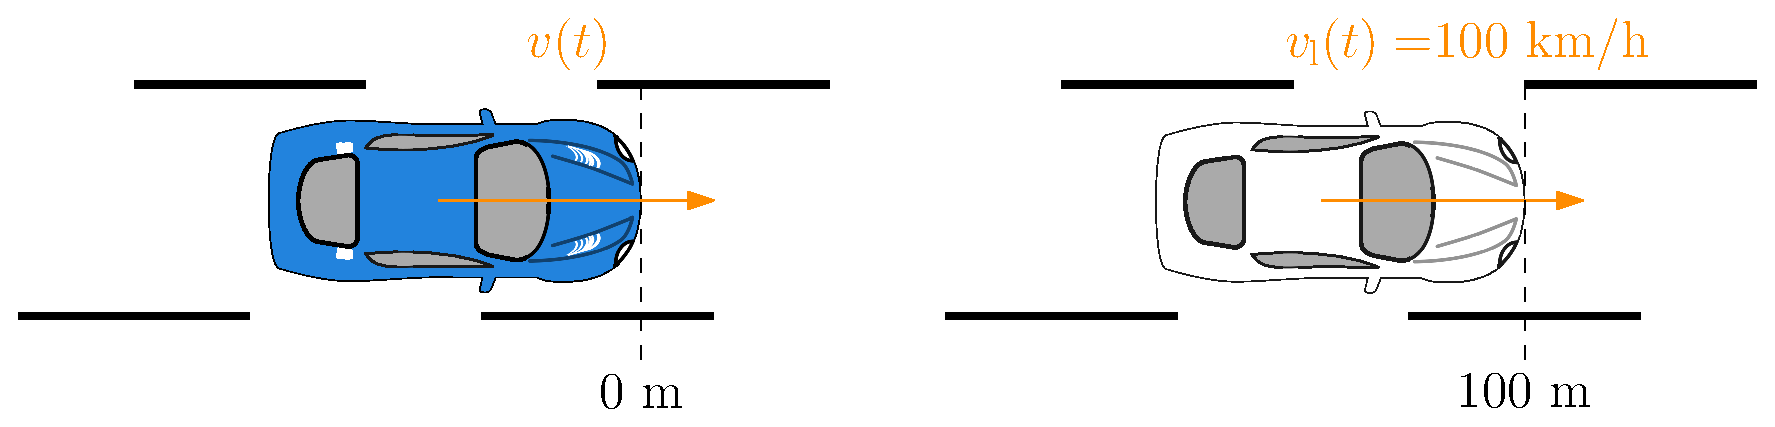
\includegraphics[width=.95\textwidth]{basic_2_car.eps}
		\caption{Basic setup with 2 cars}
		\label{fig:basic2car}
	\end{figure}
	The leading car has a constant $100$ km/h velocity. The following car which is modeled with IDM has an initial velocity of $100$ km/h as well. The parameters of following car can be seen in Table \ref{table:idm_params}
	\begin{figure}[ht]
		\begin{center}
			\begin{tabular}{ |c|c|c| }
				\hline
				$a_{\rm max}$ & $1.5$ & $\rm m/s^2$ \\
				$b_{\rm max}$ & $1.67$ & $\rm m/s^2$ \\
				$v_{\rm d}$ & $130$ & km/h \\
				$T$ & $1.8$ & s \\
				$h_0$ & $2$ & m \\
				$\rm \delta$ & $4$ & - \\
				$L$ & $4.5$ & m \\
				\hline
			\end{tabular}
		\end{center}
		\caption{Intelligent Driver Model parameters}
		\label{table:idm_params}
	\end{figure}